\chapter{RoCEv2的ClickNP实现}
\section{对RoCEv2协议进行抓包分析}
为了充分了解RoCEv2协议,我们利用微软亚洲研究院程鹏研究员基于NetDirect开发的ndping、ndrping工具发送RoCEv2包,
并使用IbDump工具对其进行抓包,用Wireshark进行分析。
\begin{figure}[htbp]
\centering
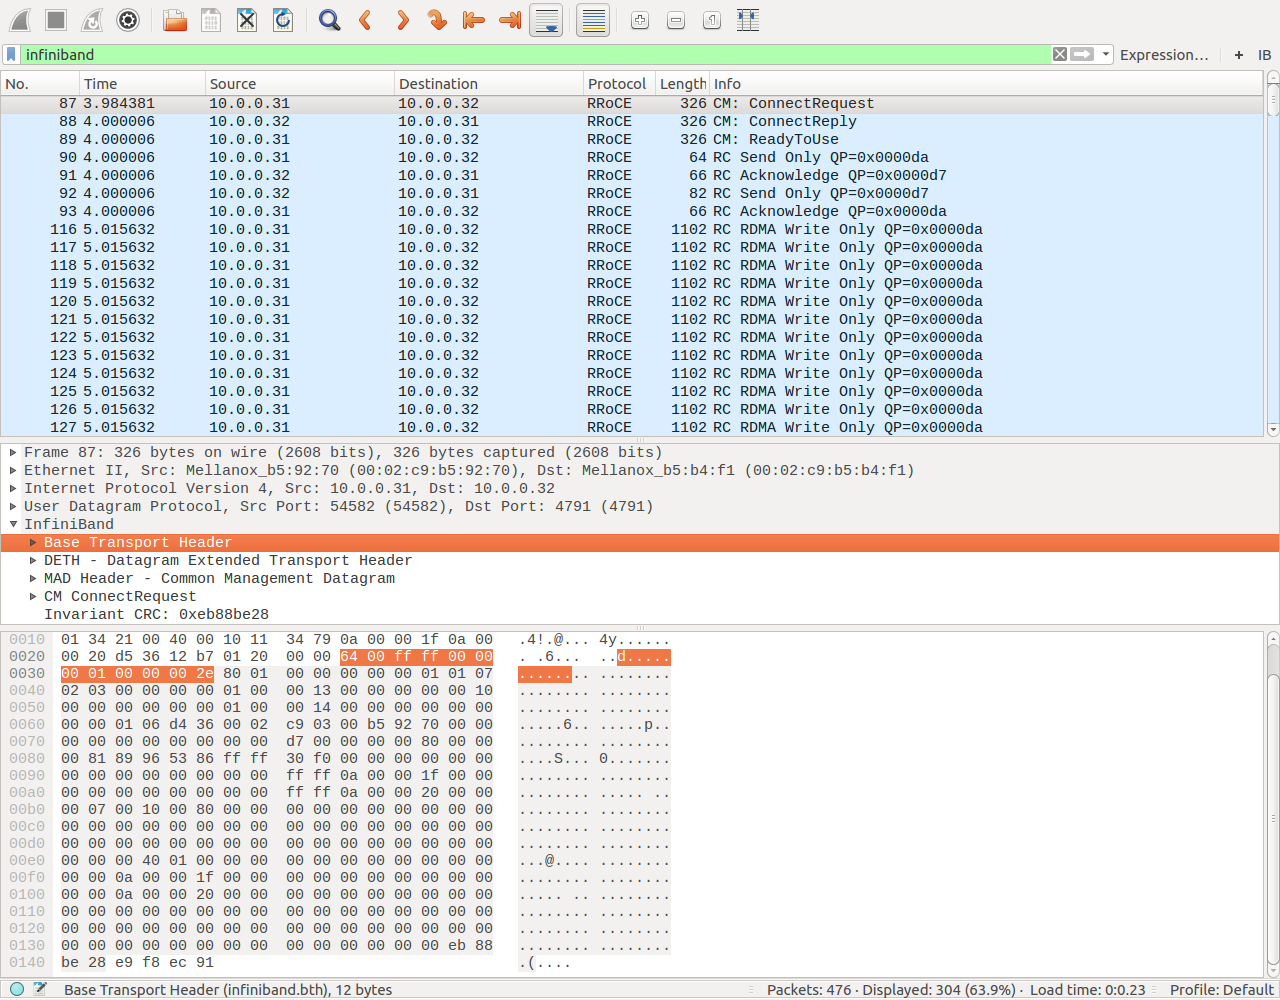
\includegraphics[width=4in]{capture}
\caption{利用Wireshark抓包分析} \label{fig:capture}
\end{figure}

我们的实验在与同一交换机相连的两台之间进行,期间基本不存在丢包的情况,
所以初期我们只能抓到无丢包情况下的包。

为了解决这一问题,我基于ClickNP平台开发了丢包器,能够在用户的控制下,以一定的概率丢包。
将丢包逻辑写入FPGA,将主机与交换机之间用FPGA串联,即可在FPGA上将包拦截下来。

将丢包率调整为10\%左右时,可以较好地观察到丢包与重传时所发的包。

在抓包的过程中,我们发现一些根据协议本应出现的包没有被观察到,
并据此猜测IbDump没有将流经网卡的包全部记录下来。

为了验证这一猜测,我们改在FPGA上抓包。在丢包器的下游增设抓包器,在记录包的同时将其发出。

在使用FPGA抓包的过程中,我们发现当发包频率加快时,会出现阻塞情况。
这是因为抓包器将包记录在主机上需要通过PCIe接口发送数据,
而PCIe接口的数据带宽低于FPGA网卡的带宽,因此缓冲区会被迅速写满,随后不再响应网卡的输入请求。

为了解决这一问题,我对ndping、ndrping的代码进行了修改,将原有的连续发送RDMA请求改为有时间间隔地发送RDMA请求。
虽然在请求长度较大时仍然会出现阻塞情况,但因为我们在FPGA上的抓包实验侧重于对丢包情况进行分析,
因此不需要发送长度太大的RDMA请求。

实验表明,FPGA的抓包结果中确实出现了之前IbDump没有记录下来的包,
这证实了我们的猜测,也验证了我们对于RoCEv2协议的初步理解。

在IbDump与FPGA两个抓包工具获取到的日志基础上进行分析,使我们加深了对RoCEv2协议的认识。

\begin{figure}[htbp]
\centering
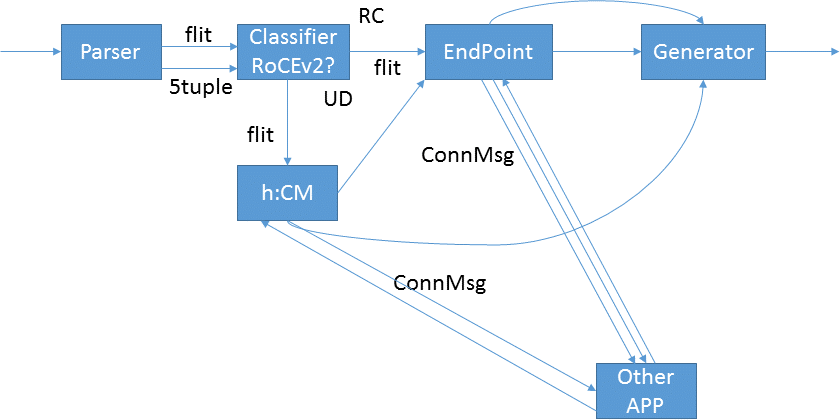
\includegraphics[width=4in]{roce}
\caption{RoCEv2各元件及其连接关系} \label{fig:roce}
\end{figure}

\begin{figure}[htbp]
\centering
\lstinputlisting[caption=RoCEv2项目的ClickNP配置文件, label=code:rocecfg]{code/RoCE.cfg}
\end{figure}

\begin{figure}[htbp]
\centering
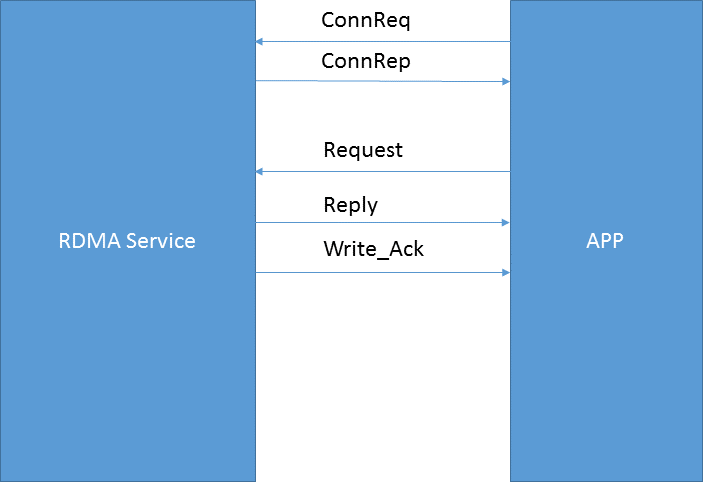
\includegraphics[width=4in]{roceapi}
\caption{应用程序与适配器之间的5条通道} \label{fig:roceapi}
\end{figure}
\section{项目实现}
\subsection{总体设计}
RoCEv2项目包含如下元件:
\begin{description}
\item[RoCE\_Classifier包分类器]将收到的包进行分类,将连接相关请求转发至连接管理器,将数据请求转发至适配器。
\item[RoCE\_Connector连接管理器]根据连接请求,建立、维护、断开连接。
\item[应用程序]向适配器发起应用RDMA请求。
\item[RoCE\_Endpoint适配器]与应用程序交互,将用户的请求转发至包生成器,并向应用程序发送反馈。
\item[RoCE\_Gen包生成器]将连接管理器和适配器发来的请求翻译为网络协议包。
\end{description}

图~\ref{fig:roce} 展示各元件间的连接关系,其配置文件如代码~\ref{code:rocecfg} 所示。

应用程序与适配器之间的5条通道功能如图~\ref{fig:roceapi} 所示。

\subsection{包生成器设计}
我设计的包生成器有2个输入端口和1个输出端口。
其中输入端口1与适配器相连,输入端口2与连接管理器相连;输出端口与网卡相连。

当输入端口有收到发包请求时,包生成器根据收到的元数据填写待发送帧的各个域,
并维护其操作码及序列号两个状态,每周期处理一帧,直到最后一帧发送完毕,读取下一个请求。

值得一提的是,由于元数据帧的信息密度大于要发送的帧,
所以只要输入端有源源不断的发包请求,输出端就不会忙等,
不需要手工维护多级流水线及其缓冲区即可充分利用设备的吞吐率。

包生成器的大致框架如代码~\ref{code:rocegen} 所示。
\lstinputlisting[caption=RoCE\_Gen包生成器示意,label=code:rocegen]{code/RoCE_Gen.cl}

截至我从微软亚洲研究院离职时,包生成器已实现CM ConnectionReply、CM ReadyToUse、
Acknowledge、RC RDMA Read Request等功能,代码量不足八百行,
预计实现全部功能只需要四千行代码。

另外,看似比较大的代码量不代表程序效率低下。因为同一个分支内不存在数据依赖,
所以这些代码在FPGA中很容易实现并行化,可以认为是同时执行。
